\documentclass[12pt,a4paper]{article}

\usepackage[margin=1in]{geometry}
\usepackage[T1]{fontenc}
\usepackage[utf8]{inputenc}
\usepackage{lmodern}
\usepackage{setspace}
\usepackage{hyperref}
\usepackage{tabularx}
\usepackage{enumitem}
\usepackage{xcolor}
\usepackage{graphicx}
\usepackage{caption}

\hypersetup{
    colorlinks=true,
    linkcolor=blue,
    urlcolor=blue
}

\setstretch{1.15}
\setlength{\parskip}{0.6em}
\setlength{\parindent}{0pt}

\begin{document}

\hypersetup{pageanchor=false}
\begin{titlepage}
\centering
{\Large Republic of Tunisia\par}
\vspace{0.5cm}
{\Large IT370 Course Project Report\par}
\vspace{2cm}
{\Huge \textbf{Tunisia Heritage Quest}\par}
\vspace{0.75cm}
{\Large Android Educational Quiz Application\par}
\vspace{2cm}
\begin{tabular}{ll}
\textbf{Student:} & Mohamed Cherif Khcherif \\
\textbf{Professor:} & Najet Boughanmi \\
\textbf{Course:} & IT370 \\
\textbf{Submission Date:} & May 6, 2026 \\
\end{tabular}
\vfill
{\large Academic Year 2025--2026\par}
\end{titlepage}

\hypersetup{pageanchor=true}
\pagenumbering{roman}
\thispagestyle{empty}
\tableofcontents
\clearpage
\pagenumbering{arabic}

\section*{Abstract}
\addcontentsline{toc}{section}{Abstract}
This report presents \textit{Tunisia Heritage Quest}, an Android educational quiz application developed for the IT370 course. The project was designed to promote knowledge of Tunisian cultural and historical heritage through an interactive mobile experience. The application combines a structured quiz flow, category-based exploration, difficulty settings, persistent player statistics, and a themed user interface inspired by Tunisian visual identity. The implementation was built with Kotlin, Jetpack Compose, Room, DataStore, and Navigation Compose. This report summarizes the project objectives, architecture, implementation choices, testing process, and the controlled use of artificial intelligence during development.

\section{Introduction}
Mobile applications are an effective medium for educational engagement because they combine accessibility, interactivity, and immediate feedback. In this project, the goal was to design and implement a quiz-based Android application centered on Tunisian heritage. The app encourages users to discover monuments, cities, and cultural sites while answering multiple-choice questions supported by visual content.

The project was also an opportunity to apply modern Android development practices, including declarative UI with Jetpack Compose, state management through ViewModels, persistent local storage, and structured navigation. Beyond functionality, the project emphasized visual quality and a culturally coherent user experience.

\section{Project Objectives}
The main objectives of the project were the following:
\begin{itemize}[leftmargin=1.5em]
    \item Develop a functional Android quiz application using Kotlin.
    \item Organize the app with a clean architecture based on MVVM principles.
    \item Provide a multi-screen user flow including splash, menu, category selection, difficulty selection, quiz gameplay, and results.
    \item Store user settings and performance statistics locally.
    \item Design an interface that reflects Tunisian heritage through color, ornament, and composition.
    \item Deliver a project that is testable, maintainable, and appropriate for an academic software engineering context.
\end{itemize}

\section{Application Overview}
The final application is a single-player heritage quiz game. The player starts from a splash screen and then navigates through the main menu to select a category and difficulty level. During gameplay, each question presents an image and four possible answers. The user selects an answer, receives feedback, and proceeds through the quiz until reaching the results screen.

The implemented categories include Roman heritage, Islamic heritage, Punic and pre-Roman heritage, modern heritage, natural and mixed sites, and Tunisian cities. Different difficulty levels adjust the challenge and timer behavior. The application also includes settings such as timer enablement, sound effects, and haptic feedback.

\section{Technical Stack}
The project was implemented with the following technologies:

\begin{center}
\begin{tabularx}{\textwidth}{|l|X|}
\hline
\textbf{Component} & \textbf{Technology Used} \\
\hline
Programming language & Kotlin \\
\hline
UI toolkit & Jetpack Compose with Material 3 foundations \\
\hline
Architecture & MVVM with unidirectional state flow \\
\hline
Navigation & Navigation Compose \\
\hline
Persistence & Room database and DataStore Preferences \\
\hline
Asynchronous programming & Kotlin Coroutines and Flow \\
\hline
Image loading & Coil with bundled local assets and remote fallback \\
\hline
Testing & JUnit-based unit tests and ViewModel-focused tests \\
\hline
\end{tabularx}
\end{center}

\section{System Architecture}
The application follows a layered architecture centered on the MVVM pattern. The user interface is built with stateless or mostly stateless composables. Business and screen logic are handled inside ViewModels, which expose state to the UI through reactive flows. Repositories act as an abstraction between the ViewModels and the data sources. Local data persistence is handled through Room for player statistics and DataStore for user settings.

This structure improves maintainability by separating concerns. UI code remains focused on presentation, while data access and application logic are isolated in dedicated layers. This approach also makes the project easier to test and extend.

\section{User Interface and User Experience}
One of the most important aspects of this project was the creation of a strong visual identity. The interface was designed around a Mediterranean blue palette with gold accents, ornamental dividers, arched motifs, and heritage-inspired card layouts. The goal was not only to make the application attractive, but also to make its appearance consistent with the cultural theme of Tunisian architecture and historical landmarks.

The screens were redesigned to move away from a default Material appearance and toward a more intentional, themed presentation. Human design decisions played the main role in this process. The high-level structure of the app, the visual style, the screen hierarchy, and the UI/UX direction were defined manually. This includes the splash composition, main menu layout, category cards, difficulty cards, quiz screen balance, and results page styling.

\section{Core Features}
The project includes the following major features:
\begin{itemize}[leftmargin=1.5em]
    \item Splash screen with thematic branding.
    \item Main menu with progress summary and quiz entry point.
    \item Category selection for different types of Tunisian heritage.
    \item Difficulty selection with gameplay settings.
    \item Quiz flow with timed questions and answer validation.
    \item Result screen with score summary and replay support.
    \item Local persistence for settings and statistics.
    \item Haptic feedback and sound effects controlled by user preferences.
    \item Local image asset support for selected questions to improve reliability.
\end{itemize}

\section{Implementation Notes}
Several practical engineering decisions were made during development. The application uses a single-activity model with navigation handled by a Compose \texttt{NavHost}. Player settings are stored with DataStore, while progress-related values such as quiz statistics are stored in Room. ViewModels manage the quiz session, answer progression, timer state, and results logic.

Because online image loading was not reliable enough for delivery conditions, the project was adapted to support bundled image assets for questions. The loader first checks the packaged local assets and only uses a remote fallback when a local image is not available. This change increased reliability and made the app more suitable for demonstration.

\section{Testing}
Testing was treated as an important part of the project rather than an optional final step. The objective was to verify both correctness and stability after major UI and logic changes.

\subsection{Testing Strategy}
The testing effort focused on the following levels:
\begin{itemize}[leftmargin=1.5em]
    \item \textbf{Unit tests:} used to validate isolated logic and output behavior.
    \item \textbf{ViewModel tests:} used to check state updates, quiz progression, result calculations, and event flow.
    \item \textbf{Build verification:} used to ensure that the application compiles successfully after feature work and refactoring.
\end{itemize}

\subsection{Validation Performed}
During development, the following verification tasks were used repeatedly:
\begin{itemize}[leftmargin=1.5em]
    \item Debug build generation through Gradle.
    \item Unit test execution for logic and ViewModel behavior.
    \item Manual on-device checking of navigation flow, themed layouts, button behavior, and image display.
\end{itemize}

These tests were especially useful after changes to quiz timing, result navigation, button responsiveness, settings toggles, and local image loading.

\subsection{Testing Evidence}
To support the validation process, terminal screenshots were collected as evidence of successful verification steps. The first screenshot documents successful debug build generation, the second documents successful unit test execution, and the third shows an additional successful verification run from the development environment.

\begin{figure}[htbp]
    \centering
    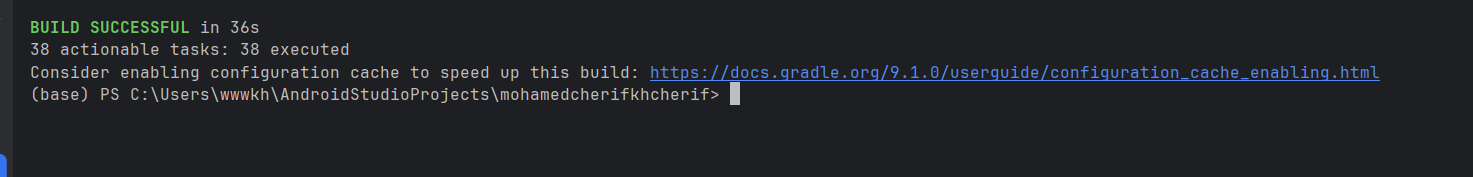
\includegraphics[width=0.9\textwidth]{report_assets/test1.png}
    \caption{Terminal output showing successful project build verification.}
\end{figure}

\begin{figure}[htbp]
    \centering
    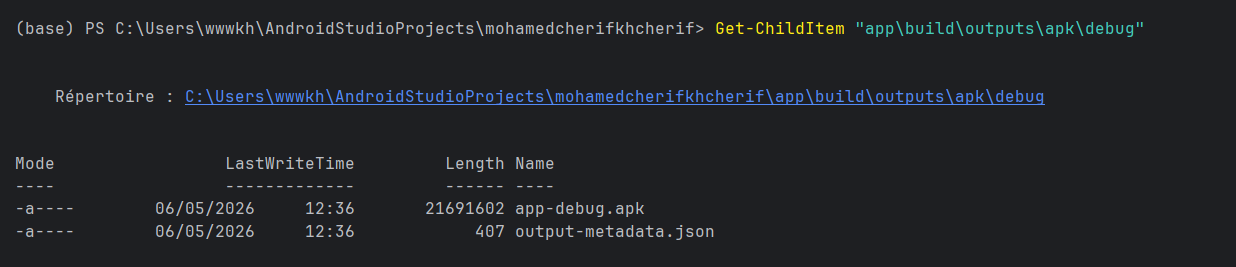
\includegraphics[width=0.9\textwidth]{report_assets/test2.png}
    \caption{Terminal output showing successful unit test execution.}
\end{figure}

\begin{figure}[htbp]
    \centering
    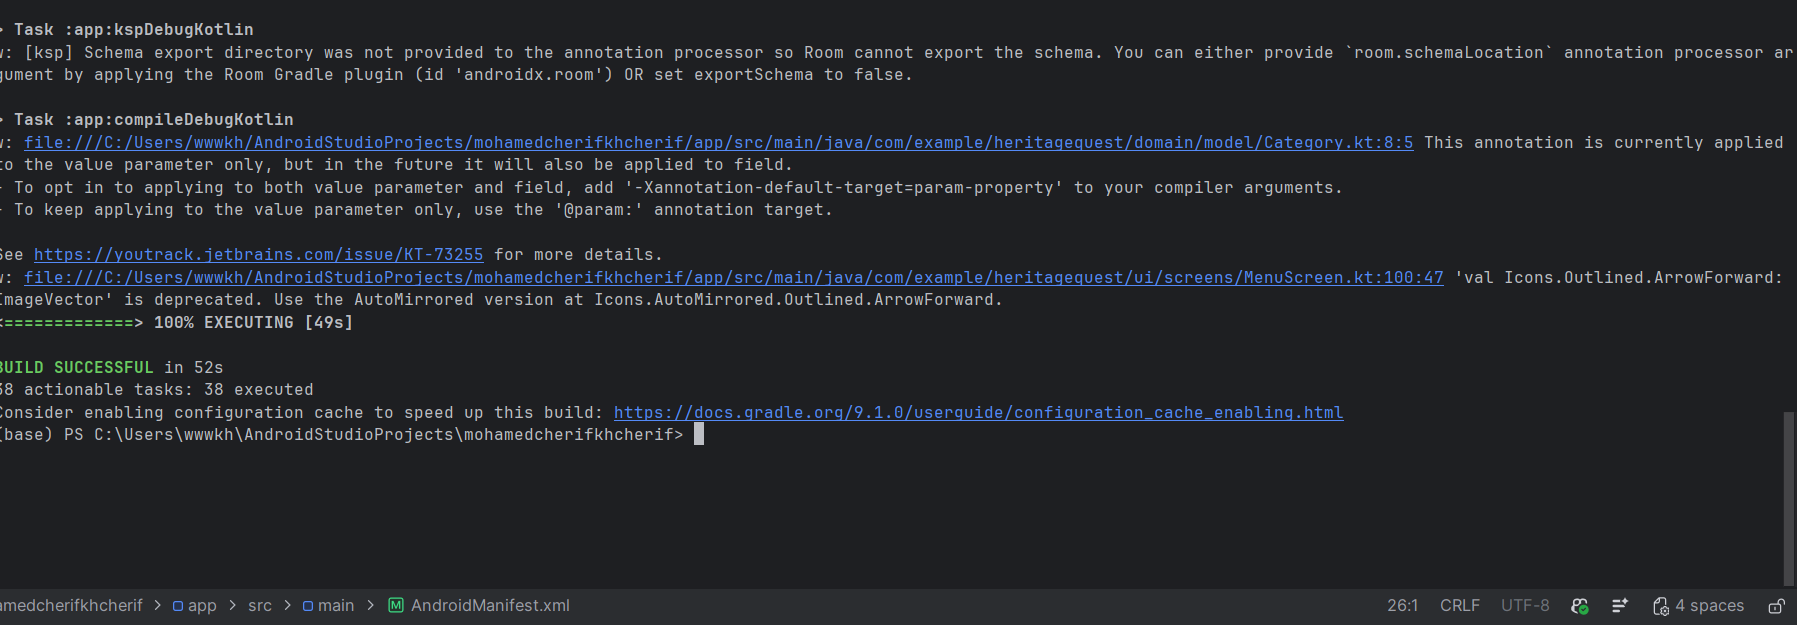
\includegraphics[width=0.9\textwidth]{report_assets/test3.png}
    \caption{Additional recorded testing evidence used during final validation.}
\end{figure}

\section{Use of Artificial Intelligence}
Artificial intelligence was used in a limited and controlled manner during this project. Its role was supportive rather than dominant.

\subsection{Tasks Assisted by AI}
AI was used for:
\begin{itemize}[leftmargin=1.5em]
    \item question generation,
    \item code review,
    \item test generation and testing support,
    \item image generation,
    \item and a small portion of code implementation.
\end{itemize}

\subsection{Tasks Led by Human Work}
The main human contribution remained central to the project. Human work covered:
\begin{itemize}[leftmargin=1.5em]
    \item the high-level design of the application,
    \item feature direction and product decisions,
    \item the UI/UX design vision,
    \item visual style selection,
    \item review of implementation quality,
    \item and final integration decisions.
\end{itemize}

In other words, AI was used as an assistant for acceleration and support, while the human role remained responsible for the conceptual direction, aesthetic choices, and major product decisions.

\section{Challenges and Solutions}
The project encountered several practical challenges. One challenge was the mismatch between the initial functional implementation and the desired UI quality. This was solved by introducing a custom themed design system and redesigning the main screens. Another challenge involved quiz image reliability. Remote loading alone was not stable enough, so the solution was to support bundled local assets for selected quiz questions. A further issue concerned responsiveness on smaller layouts, especially for action buttons, which was addressed by revising component sizing and layout behavior.

These iterations improved both usability and presentation while keeping the application aligned with the original educational objective.

\section{Conclusion}
Tunisia Heritage Quest demonstrates how modern Android development tools can be used to build an educational application with both technical structure and strong visual identity. The project integrates Kotlin, Jetpack Compose, ViewModels, Room, DataStore, and testing practices into a coherent mobile product. It also reflects a balanced workflow in which AI was used selectively for support, while the main design and UX direction remained human-driven.

Overall, the project satisfies the academic goal of producing a functional, themed, and structured Android application while offering room for future extension, such as adding more bundled images, broader test coverage, and expanded question content.

\end{document}
